\documentclass{bmstu}

\bibliography{biblio}

\usepackage{geometry} % Отступы
    \geometry{left=20mm}
    \geometry{right=10mm}
    \geometry{top=20mm}
    \geometry{bottom=20mm}


\begin{document}

\makereporttitle
    {Информатика и системы управления}
    {Программное обеспечение ЭВМ и информационные технологии}
    {лабораторной работе №~4}
    {Анализ алгоритмов}
    {}
    {}
    {Новиков~А.~А./ИУ7-52Б}
    {Строганов~Д.~В.}

\renewcommand{\contentsname}{СОДЕРЖАНИЕ} 
\tableofcontents
\setcounter{page}{2}

\begin{center}
    \textbf{ВВЕДЕНИЕ}
\end{center}
\addcontentsline{toc}{chapter}{ВВЕДЕНИЕ}

Многопоточность — это способность центрального процессора или одного из ядер в многоядерной архитектуре одновременно выполнять несколько процессов или потоков, поддерживаемых операционной системой.

В общем случае поток исполнения представляет собой последовательность инструкций, выполняемых на выделенном процессорном ядре и управляемых планировщиком операционной системы. Потоки могут приостанавливаться или блокироваться во время выполнения. Они создаются внутри процесса и совместно используют его ресурсы, такие как оперативная память и дескрипторы файлов. Такой механизм называется нативными потоками. Нативные потоки позволяют эффективно использовать системные ресурсы и выполнять несколько задач параллельно в рамках одного процесса, что существенно повышает производительность приложений ~[\cite{threads}.

\textbf{Цель лабораторной работы} --- сравнить основные принципы последовательных вычислений с параллельными на основе нативных потоков. Для достижения поставленной цели необходимо выполнить следующие задачи:

\begin{itemize}
    \item[---] описать входные, выходные данные;
    \item[---] реализовать два алгоритма для загрузки контента из $HTML$---страниц: последовательный и параллельный с использованием нативных потоков;
    \item[---] протестировать разработанные алгоритмы;
    \item[---] сравнить скорость выполнения программы в зависимости от количества используемых потоков.
\end{itemize}


\chapter{Входные и выходные данные}

Входные данные: базовый $URL$---адрес веб-сайта, число обрабатываемых страниц, количество используемых потоков (1 - для последовательного режима).

Выходные данные: файлы, содержащие полученный контент с соответствующих страниц рецептов.


\chapter{Тестирование}
В таблице ~\ref{tbl:tests} представлены функциональные тесты для разработанного
программного обеспечения. Все тесты пройдены успешно.

\begin{table}[h!]
    \begin{center}
		\begin{threeparttable}
    \caption{Описание тестовых случаев}
    \captionsetup{justification=raggedright, singlelinecheck=false}
    \label{tbl:tests}
    \begin{tabular}{|c|p{6cm}|p{6cm}|c|}
        \hline
        \textbf{№} & \textbf{Входные данные} & \textbf{Ожидаемый результат} & \textbf{Результат теста} \\
        \hline
        1 & Корректный URL, 1 поток (тестирование последовательного режима) & Директория с текстами рецептов \texttt{recipes} & Пройден \\
        \hline
        2 & Корректный URL, 16 потоков (тестирование параллельного режима) & Директория с текстами рецептов \texttt{recipes} & Пройден \\
        \hline
        3 & Пустой URL & Вывод сообщения об ошибке, повторный запрос ввода & Пройден \\
        \hline
        4 & Некорректный URL & Вывод сообщения об ошибке, повторный запрос ввода & Пройден \\
        \hline
        5 & Не положительное число страниц & Вывод сообщения об ошибке, повторный запрос ввода & Пройден \\
        \hline
        6 & Не положительное число потоков & Вывод сообщения об ошибке, повторный запрос ввода & Пройден \\
        \hline
    \end{tabular}
    \end{threeparttable}
    \end{center}
\end{table}




\chapter{Описание исследования}
В ходе исследования требуется сравнить скорость выполнения программы в зависимости от количества используемых потоков. Замеры проводились при обработки 5 страниц, каждая из которых содержала 30 рецептов.

\section{Технические характеристики}
Технические характеристики используемого устройства:
\begin{itemize}
    \item[---] операционная система --- Ubuntu Linux x86\_64 ~[\cite{Ubuntu}
    \item[---] память --- 16 Гб.
    \item[---] процессор --- AMD Ryzen 5 5500U (6x2.10 ГГц) ~[\cite{AMD}
\end{itemize}

\section{Полученные результаты}

В таблице ~\ref{tbl:time_measurements1} приведено время выполнения
программного обеспечения в миллисекундах (далее --- мс). На рисунке
~\ref{fig:image1} показана зависимость времени работы от количества
потоков без изменений количества обрабатываемых страниц сайта.

\begin{table}[h]
	\begin{center}
		\begin{threeparttable}
		\captionsetup{justification=raggedright,singlelinecheck=off}
		\caption{Время работы от количества потоков (в миллисекундах)}
		\label{tbl:time_measurements1}
                    \begin{tabular}{|r|r|}
                        \hline
                        Количество потоков & Время работы\\
                        \hline
                        1 & 125,979 \\
                         \hline
                        2 & 69,736 \\
                         \hline
                        4 & 35,228 \\
                         \hline
                        8 & 17,600 \\
                         \hline
                        16 & 9,346 \\
                         \hline
                        32 & 4,577 \\
                         \hline
                    \end{tabular}
		\end{threeparttable}
    \end{center}
\end{table}

\begin{figure}[h!]
    \centering
    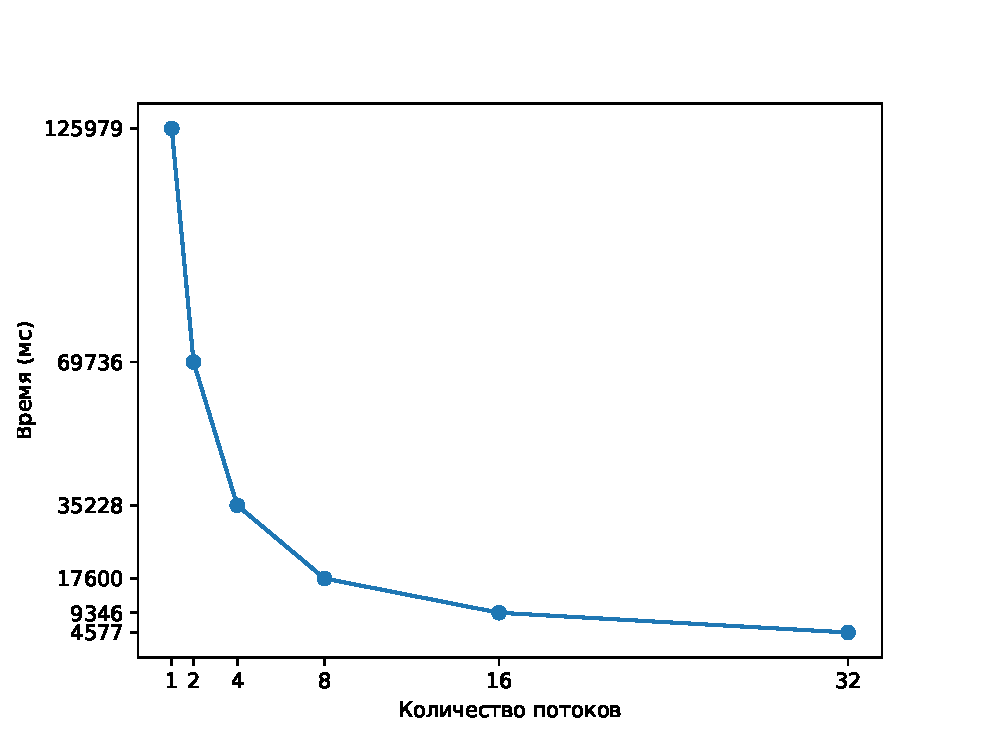
\includegraphics[width=0.8\textwidth]{img/Figure_1.eps}
    \caption{Зависимость времени выполнения программы от количества потоков}
    \label{fig:image1}
\end{figure}

В таблице ~\ref{tbl:time_measurements2} приведено время выполнения в зависимости
от количества обрабатываемых страниц. В отличие от предыдущего исследования,
в таблице ~\ref{tbl:time_measurements2} отсутствует зависимость от количества
потоков.

\clearpage

\begin{table}[h]
	\begin{center}
		\begin{threeparttable}
		\captionsetup{justification=raggedright,singlelinecheck=off}
		\caption{Время работы программы в зависимости от количества обрабатываемых страниц (в мс)}
		\label{tbl:time_measurements2}
                \begin{tabular}{|r|r|r|}
			\hline 
			& \multicolumn{2}{c|}{Время для реализации} \\
                        \cline{2-3}
			Количество страниц & 1 поток & 16 потоков\\
			\hline
                        1 & 8,951 & 2,266 \\
                         \hline
                        2 & 16,315 & 3,205 \\
                         \hline
                        3 & 25,555 & 3,559 \\
                         \hline
                        4 & 34,707 & 4,623 \\
                         \hline
                        5 & 40,462 & 5,422 \\
                         \hline
		\end{tabular}
		\end{threeparttable}
    \end{center}
\end{table}

На рисунке ~\ref{fig:image2} показана зависимость времени работы от количества
обрабатываемых страниц.

\begin{figure}[h!]
    \centering
    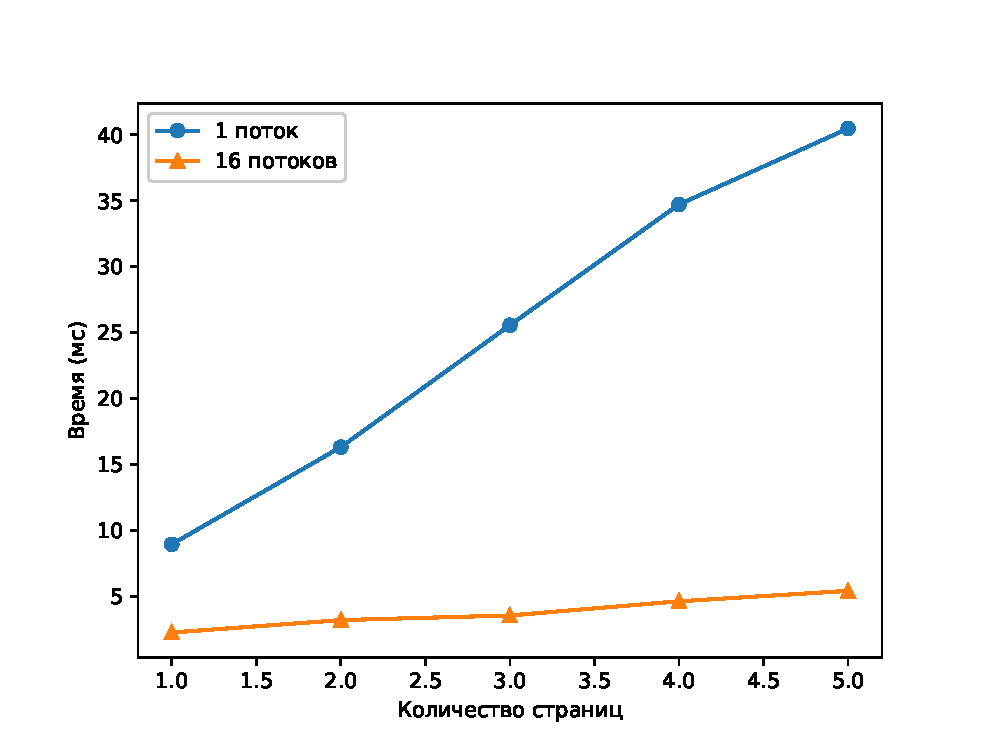
\includegraphics[]{img/Figure_2.eps}
    \caption{Зависимость времени работы программы от числа страниц}
    \label{fig:image2}
\end{figure}



\clearpage


\section{Вывод}
Исследование показало, что однопоточная реализация программы работает значительно медленнее по сравнению с многопоточной версией. При фиксированном количестве потоков и увеличении числа обрабатываемых страниц время выполнения однопоточной программы примерно в 8 раз больше, чем у 16-поточной версии.

При увеличении количества потоков и фиксированном числе обрабатываемых страниц время выполнения сокращается приблизительно в 2 раза при удвоении числа потоков.



\begin{center}
    \textbf{ЗАКЛЮЧЕНИЕ}
\end{center}
\addcontentsline{toc}{chapter}{ЗАКЛЮЧЕНИЕ}

Цель работы достигнута: получен навык организации параллельных вычислений по конвейерному принципу.

\vspace{5mm}

В ходе выполнения данной лабораторной работы были решены следующие задачи:
\begin{itemize}
	\item[---] описаны входные, выходные данные программы;
	\item[---] реализован алгоритм обработки данных с использованием конвейерной обработки;
	\item[---] протестирован разработанный алгоритм по методологии черного ящика;
        \item[---] проанализирована информация, полученная из лог-файлов.
\end{itemize}
\makebibliography



\end{document}